Ho scelto di realizzare una gerarchia di entità che potesse comprendere tutti i componenti importanti ai fini della partita. Per questo ho creato il trait Entity, che rappresenta una qualsiasi entità sulla mappa di gioco, dotata di una posizione propria. Il trait viene poi esteso per distinguere tra le entità che occupano una posizione fissa (Collectible, Obstacle, componenti dell'arena) e quelle che invece possono muoversi (MovableEntity): queste ultime possiedono metodi per avanzare di posizione all'interno dell'arena, data una direzione di movimento. Il trait EnemyCharacter rappresenta i nemici, mentre il trait LivingEntity viene applicato alle entità dotate di un proprio punteggio che ne rappresenta la vita a disposizione (Hero, EnemyCharacter).
\begin{figure}[H]
  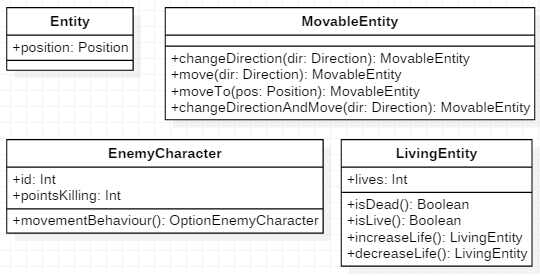
\includegraphics[width=15cm]{res/entitiesTraits.png}
  \caption{Trait delle entità del gioco}
  \label{entityTraits}
\end{figure}